\documentclass[12pt,a4paper]{ctexart}
\usepackage{geometry}
\geometry{left=2.5cm,right=2.5cm,top=2.5cm,bottom=2.5cm}
\usepackage{listings}
\usepackage{xcolor}
\usepackage{graphicx}
\usepackage{booktabs}
\usepackage{amsmath}
\usepackage{tikz}
\usetikzlibrary{automata,positioning,arrows}

\lstset{
  basicstyle=\small\ttfamily,
  keywordstyle=\color{blue}\bfseries,
  commentstyle=\color{gray}\itshape,
  stringstyle=\color{red},
  numbers=left,numberstyle=\tiny\color{gray},
  frame=single,rulecolor=\color{black!30},
  breaklines=true,breakatwhitespace=true,
  language=C++
}

\title{\textbf{编译器设计专题实验报告}\\[0.5em]实验一：DFA模拟器实现}
\author{张凌曜 \quad 2234214014 \quad 计算机2306}
\date{}

\begin{document}
\maketitle
\thispagestyle{empty}

\section{实验目的}
用C++写一个DFA模拟程序，能从文件读取DFA五元组定义，判断DFA合法性，枚举长度不超过$N$的所有合法字符串，以及模拟字符串识别过程。

\section{实验原理}
DFA就是五元组$(Q, \Sigma, \delta, q_0, F)$，分别是状态集、字符集、转移函数、初态和接受状态集。识别字符串时从初态出发，按输入字符逐步转移，最终落在接受状态就算接受。

枚举合法字符串我用了BFS：从初态开始逐层扩展所有可能的字符组合，凡是到达接受状态的路径就对应一个合法字符串。

\section{实验过程}

\subsection{DFA状态图}
测试用的DFA如图\ref{fig:dfa}，用五元组写出来就是：
\[Q=\{1,2,3,4\},\quad \Sigma=\{a,b\},\quad q_0=1,\quad F=\{3\}\]
转移函数$\delta$：$\delta(1,a)=2$，$\delta(2,b)=3$，$\delta(2,a)=4$，$\delta(4,b)=3$。

\begin{figure}[h]
\centering
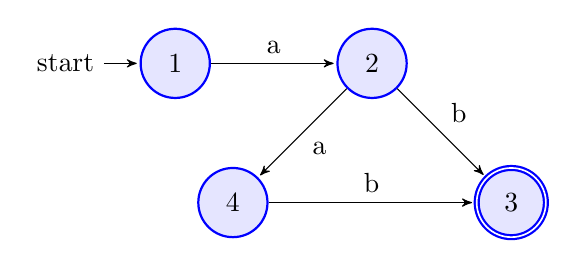
\begin{tikzpicture}[->,>=stealth',shorten >=1pt,auto,node distance=2.5cm,
  every state/.style={fill=blue!10,draw=blue,thick}]
  \node[state,initial] (1) {1};
  \node[state] (2) [right of=1] {2};
  \node[state,accepting] (3) [below right of=2] {3};
  \node[state] (4) [below left of=2] {4};
  \path (1) edge node {a} (2);
  \path (2) edge node {b} (3);
  \path (2) edge node {a} (4);
  \path (4) edge node {b} (3);
\end{tikzpicture}
\caption{测试DFA状态转换图}
\label{fig:dfa}
\end{figure}

\subsection{输入文件格式}
DFA五元组存在\texttt{dfa\_in1.dfa}里，一行一类信息，比较直观：

\begin{lstlisting}[language={}]
a b           % 字符集
1 2 3 4       % 状态集
1             % 开始状态
3             % 接受状态集
1 a 2         % 转换表
2 b 3
2 a 4
4 b 3
\end{lstlisting}

\subsection{实现要点}
程序里用\texttt{map<pair<string,char>, string>}存转移表，查表方便。合法性检查就是验证初态在状态集里、接受状态集非空且包含于状态集。

字符串识别部分，逐字符查表做转移，同时把经过的状态记到vector里输出路径。BFS枚举用的是队列，队列元素是当前字符串、当前状态和路径，每次取出一个元素尝试扩展所有字符，长度不超过$N$且到达接受状态就保存。

关于BFS的复杂度：每一层最多扩展$|\Sigma|^k$个字符串（$k$是当前层深度），如果DFA里有环的话合法字符串数量会随$N$指数增长，队列的内存消耗也会跟着涨。本实验$N$取3所以没问题，但如果$N$比较大（比如20以上）就得考虑内存限制了。

\section{测试结果}

\subsection{合法性检查与异常测试}
程序启动后会自动打印DFA信息并进行合法性检查：

\begin{center}
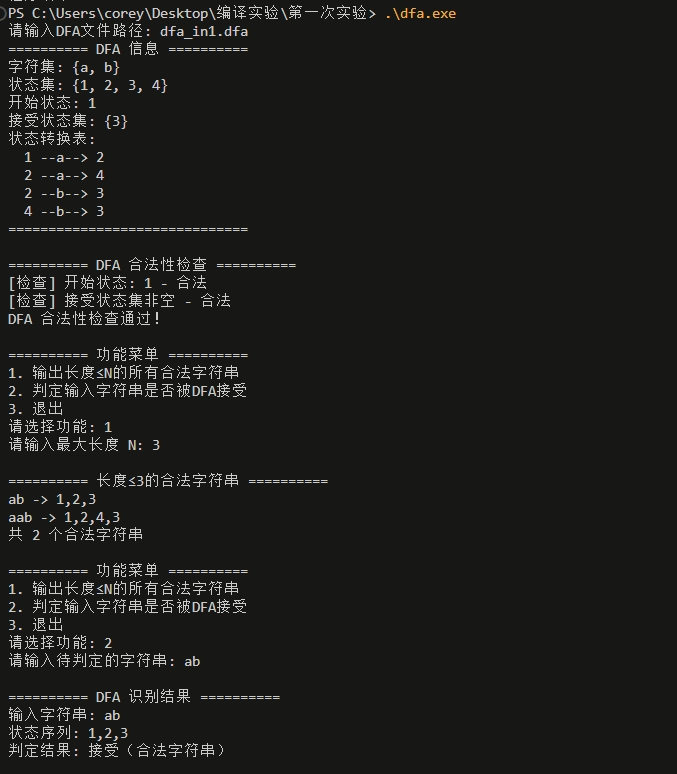
\includegraphics[width=0.9\textwidth]{image/1.png}
\end{center}

除了正常识别之外，也测了几个异常情况：

\begin{table}[h]
\centering
\begin{tabular}{ll}
\toprule
异常输入 & 程序行为 \\
\midrule
初态不在状态集中（如$q_0=5$） & 报错：开始状态不合法 \\
接受状态不在状态集中 & 报错：接受状态集包含非法状态 \\
转移表含字符集外的字符 & 该条转移被忽略，不影响运行 \\
\bottomrule
\end{tabular}
\end{table}

\subsection{字符串识别}

\begin{table}[h]
\centering
\caption{字符串识别结果}
\begin{tabular}{ccc}
\toprule
输入 & 状态序列 & 结果 \\
\midrule
ab & 1,2,3 & 接受 \\
a & 1,2 & 拒绝 \\
aab & 1,2,4,3 & 接受 \\
b & -- & 拒绝 \\
\bottomrule
\end{tabular}
\end{table}

输入$ab$时状态从1经$a$到2再经$b$到3（接受状态），没问题。输入$a$停在状态2不是接受状态，拒绝。输入$b$第一步就没有转移，直接拒绝。

枚举最大长度$N=3$时输出\texttt{ab}和\texttt{aab}两个字符串，手算验证过确实就这两个。

\begin{center}
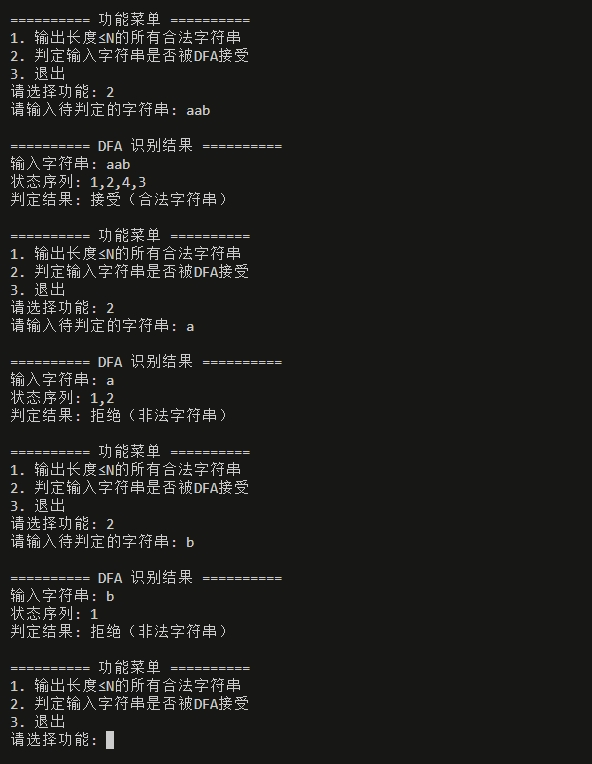
\includegraphics[width=0.9\textwidth]{image/2.png}
\end{center}

\section{实验总结}
写BFS枚举的时候踩了个坑：一开始用\texttt{const auto\&}引用队列里的vector元素，结果\texttt{push\_back}触发vector扩容后引用就悬空了，程序直接崩。改成值拷贝就没事了，C++容器迭代器失效这块确实得注意。

整体来说这个实验难度还行，文件输入格式设计比较直观，两个功能都能跑通。

\appendix
\section{附录：代码仓库}
本实验的全部源码、报告及Web演示平台已托管至GitHub：

\texttt{https://github.com/yaossss123/compilation-web}

\end{document}
